
\documentclass{article}
\usepackage{graphicx} % for figures
\usepackage[margin=1.5in]{geometry} % 1-inch page margins
\usepackage{amsmath} % additional math symbols
\usepackage{hyperref} % embeding hypertext URLs (web links)
\usepackage{enumitem}
\renewcommand{\arraystretch}{2}
%\renewcommand{\theenumi}{\Alph{enumi}}
\usepackage{caption}
\usepackage{subcaption}
\usepackage{multirow}

\begin{document}

\title{HW \#4: Football trajectory and Euler's Method}
\author{Aaron Deich}
%\date{24 September 2014} % if you want to set the date manually

\maketitle

Following the guidelines of the HW \#4 pseudocode, I wrote a Python program \texttt{balle.py} which computes and plots the trajectory of a football, both with the exact, analytic solution (in vacuum) and with Euler's method (both in vacuum and then with air resistance). If it's helpful, I'm storing my code in a GitHub repository at \url{https://github.com/adeich/Physics-240-Spring-2015/tree/master/HW4}



\begin{figure}[h!]
   \centering
    \includegraphics[width=1.1\textwidth]{20_45_no_air.png}
     \caption{I first checked that my Euler's Method integrator (with no air resistance) agrees with the analytic vacuum trajectory by plotting both together: There is fairly good agreement between the two. Here, $v_0$ = 20 m/s and $\theta_0$ = 45 degrees.}

\end{figure}



\begin{figure}[h!]  
  \centering
    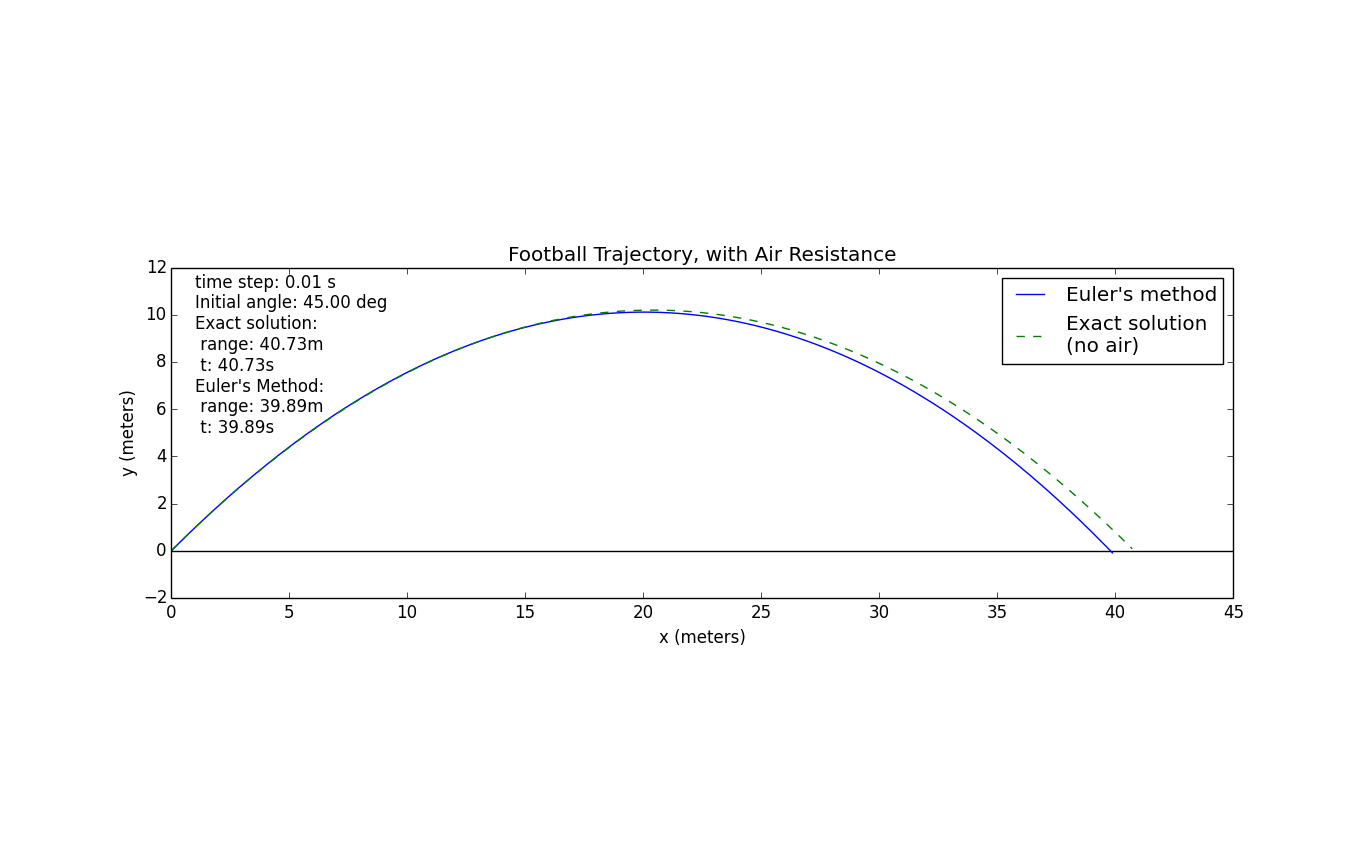
\includegraphics[width=1.1\textwidth]{20_45_yes_air.png}
    \caption{Part (a). Here is a typical football throw, with $v_0$ = 20 m/s and $\theta_0$ = 45 degrees. The solid line show the Euler's method trajectory (with air resistance) and the dashed line shows the vacuum, analytic trajectory for the same initial throw. The range of the throw, with and without air resistance, is 39.9m and 40.7m, respectively.}
\end{figure}


\begin{figure}[h!]
   \centering
    \includegraphics[width=1.1\textwidth]{30_30_yes_air.png}
     \caption{Here is the same calculation but now with initial conditions of a typical field goal kick: $v_0$ = 30 m/s and $\theta_0$ = 30 degrees. Again, the range, with and without air resistance, is 76.2m and 79.5m, respectively. In reality, this kick tends to only have a range of 55m. My guess as to a large reason why my calculation is so much greater is that mine assumes the football has a perfect spiral spin; with kicks this is never the case and the ball would certainly have a much bigger cross section.}
\end{figure}

 Again, so we can see the effect of air resistance, the vacuum-analytic trajectory is plotted as well.

%\begin{tabular}{ l| l| l|  l| l| l }
%  Dwarf Galaxy    & RA              & DEC        & z              & i-band mag & petroRad   \\ \hline
%  CGCG 015-033 & 193.50786 &  -1.50834 & 0.003821 & 14.05          & 10.50 $\pm$ 0.146 
%\end{tabular}


%\begin{align*}
%\theta_{sep} &= \cos^{-1}(\sin(d1)\sin(d2) + \cos(d1)\cos(d2)\cos(r1 - r2)) \\
% &= 31.1 \mathrm{'}
%\end{align*}

\end{document}